\documentclass[%
master,         % тип документа
subf,           % подключить и настроить пакет subfig для вложенной нумерации рисунков
href,           % подключить и настроить пакет hyperref
colorlinks=true % цветные гиперссылки
%,times         % шрифт Times как основной
%,fixint=false  % отключить прямые знаки интегралов
]{disser}

\usepackage[
a4paper, mag=1000,
left=2.5cm, right=1cm, top=2cm, bottom=2cm, headsep=0.7cm, footskip=1cm
]{geometry}
\usepackage[T2A]{fontenc}
\usepackage[utf8]{inputenc}
\usepackage[english,russian]{babel}
\usepackage{algorithm}
\usepackage{longtable}
\usepackage{float}
\usepackage{cleveref}
\usepackage{footnote}
\usepackage{totcount}
\usepackage{algpseudocode}
\usepackage{amssymb,amsthm}
\usepackage{amsmath}
\usepackage{mathtools}
\usepackage[export]{adjustbox}
\usepackage{graphicx}
\ifpdf\usepackage{epstopdf}\fi

\newtheorem{theorem}{Theorem}
\newtheorem{definition}[theorem]{Определение}

% Номера страниц снизу и по центру
\pagestyle{footcenter}
\chapterpagestyle{footcenter}

% Точка с запятой в качестве разделителя между номерами цитирований
%\setcitestyle{semicolon}

% Использовать полужирное начертание для векторов
\let\vec=\mathbf

% Включать подсекции в оглавление
\setcounter{tocdepth}{2}
\graphicspath{{fig/}}
\captionsetup[subfigure]{labelformat=parens, labelsep=space}
\bibliographystyle{gost705}
\regtotcounter{page}
\regtotcounter{figure}
\regtotcounter{table}

\newtotcounter{figuresnum}
\def\oldfigure{} \let\oldfigure=\figure
\def\figure{\stepcounter{figuresnum}\oldfigure}

%\newtotcounter{tablesnum}
%\def\oldtable{} \let\oldtable=\table
%\def\table{\stepcounter{tablesnum}\oldtable}

\newcommand{\bb}[1]{\mathbb{#1}}
\newcommand{\q}[1]{``#1''}
\DeclarePairedDelimiter\abs{\lvert}{\rvert} % absolute value
\DeclarePairedDelimiter\floor{\lfloor}{\rfloor} % floor

\newtheorem{theo}{Теорема}
\newtheorem{lem}[theo]{Лемма}
\newtheorem{define}[theo]{Определение}
\newtheorem{prob}[theo]{Проблема}
\newtheorem{task}[theo]{Задача}
\newtheorem{example}{Пример}

\begin{document}
\algnotext{EndFor}
\algnotext{EndIf}
\algnotext{EndWhile}
\newcommand*\thesubfloatfigure{\themainfigure\alph{subfloatfigure}}

\institution{
  \begin{figure}
    \centering
    
\includegraphics[scale = 0.4]{fig/au_logo.jpg}
  \end{figure}
}

% Имя лица, допускающего к защите (зав. кафедрой)

\apname{А.В. Омельченко}

\title{\vspace{-1.5ex}\bf{ДИССЕРТАЦИЯ}\\[-14pt]\textnormal{НА СОИСКАНИЕ УЧЕНОЙ СТЕПЕНИ}\\МАГИСТРА}

\topic{Реконструкция филогенетических деревьев на основе данных о перестройках и событиях вставок и удалений генов\vspace{-5.5ex}}

% Автор
\author        {Н.М. Карташов} % ФИО
\coursenum {03.04.01} % Номер направления
\course       {Прикладные математика и физика}

% Научный руководитель
\sa      {М. А. Алексеев}
\sastatus{PhD, доцент}
% Рецензент
\rev      {А. В. Банкевич}
\revstatus{м.н.с.}


% Город и год
\city{Санкт-Петербург}
\date{\number\year}
\maketitle
\pagebreak

\thispagestyle{empty}
\setcounter{page}{1}

\section*{Благодарности}
\noindent

Спаибо Павлу Авдееву, Антону Банкевичу (СПбАУ), Максиму Алексееву (GWU) и Yu Lin (EPFL).

\pagebreak

\thispagestyle{empty}
\setcounter{page}{1}

\section*{Реферат}
\noindent
С. \total{page},  рис. \total{figuresnum}, табл. \total{table}.

В данной работе представлен алгоритм восстановления деревьев,

\textbf{Ключевые слова}: брейкпоинт-граф, филогенетические паттерны, восстановление филогенетических деревьев.

\pagebreak


% Содержание
\tableofcontents
% Введение
\intro

Все биологические дисциплины согласны в том, что биологические виды имеют общую историю.
Для выбранной группы организмов данная история может быть представлена в виде филогенетического дерева.
Анализ филогенетических деревьев и предковых геномов является одним из главных инструментов эволюционной биологии.
Восстановление филогенетических деревьев на сегодняшний день может проводиться на основе данных секвенирования.
Новые технологии секвенирования позволяют получать большое количество данных секвенирования относительно дешево и быстро,
потому особенно важно уметь восстанавливать филогенетические деревья на их основе быстро и точно.
Знание филогенетического дерева полезно в ряде приложений, его получение делает возможным восстановление предковых геномов с высокой точностью,
облегчает точную сборку секвенированных геномов, дает понимание о том, как шел процесс эволюции.

На данный момент существует множество программных средств решающих задачу восстановления филогенетических деревьев на основе данных
секвенирования, отличающихся как в подходах к решению задачи, так и в информации используемой для восстановления,
в данной работе представлены два алгоритма, решающие задачу восстановления деревьев из разделений, информация о которых получается из брейкпоинт-графа,
а также рассмотрен метод поиска способов извлечения филогенетической информации из брейкпоинт-графа.
Алгоритмы реализованы как часть программного пакета MGRA2 на языке C++ и доступен под лицензией GNU GPL v2.0.

Диссертация состоит из трёх глав.
В первой главе описывается постановка задачи и дается обзор существующих методов.
Вторая глава посвящена описанию методов получения филогенетической информации и алгоритмов восстановления деревьев на ее основе.
Третья глава содержит сравнение реализованных методов с известными на тестовых данных.

% Глава 1
\chapter{Обзор предметной области, существующих решений и постановка проблемы}

\section{Обзор предметной области}
Общеизвестно, что молекула ДНК в процессе эволюции может меняться.
Изменения происходящие в молекуле ДНК можно разделить на две группы:
\begin{enumerate}
  \item Точечные (замены, вставки и удаления на уровне отдельных нуклеотидов)
    \begin{itemize}
      \item Замена - замена одного нуклеотида в цепи на другой
      \item Вставка - добавление нового нуклеотида в цепь
      \item Удаление - удаление нуклеотида из цепи
    \end{itemize}
  \item Структурные (перестройки на уровне отдельных сегментов молекулы ДНК)
    \begin{itemize}
      \item Инверсия - разворот части цепи и встраивание его на то же самое место
      \item Вставка - вставка нового фрагмента цепи между существующими
      \item Удаление - удаление фрагмента цепи
      \item Слияние - слияние двух разных хромосом в одну
      \item Разделение - разбиение хромосомы на две новых
      \item другие
    \end{itemize}
\end{enumerate}

В ходе исследования эволюции выдвигалось две гипотезы о местах в которых происходят структурные перестройки: \q{случайная} и \q{хрупкая}.
Первая утверждает, что границы блоков, над которыми происходят структурные перестройки, расположены по геному случайным образом~\cite{ohno1973ancient},
когда последняя утверждает,
что перестройки не могут происходить в случайных местах генома~\cite{pevzner2003human}~\cite{webber2005hotspots}~\cite{peng2006fragile}.
В ходе исследований последних 20 лет ученые пришли к консенсусу, что перестройки происходят не в случайных местах генома,
но в процессе эволюции в геноме появляются и исчезают хрупкие регионы~\cite{alekseyev2010comparative}.
На основе этого факта можно ввести понятие \textit{блоков синтении}~\cite{renwick1971mapping}.

\begin{define}{Блоки синтении} \\
  В молекуле ДНК существуют консервативные регионы, называемые блоками синтении (синтенными блоками),
  геномные перестройки в которых маловероятны.
\end{define}

В данной работе геном будет рассматриваться в виде набора хромосом,
где каждая хромосома состоит из набора блоков синтении и молекула ДНК подвержена только структурным изменениям.

Хромосомы в геноме могут быть циклическими и линейными.
Другими словами, каждая хромосома представляется в виде перестановки над синтенными блоками.
Для того чтобы определить понятие \textit{перестановки над блоками синтении} введем понятие \textit{знаковой перестановки}.
\begin{define}{Знаковая перестановка} \\
  Знаковая перестановка над множеством элементов $\bb{B}$ - перестановка над элементами из $\bb{B}$, в которой каждый элемент имеет знак.
\end{define}
Имея определения знаковой перестановки необходимо определить множество ее элементов - \textit{множество блоков синтении}.
\begin{define}{Множество блоков синтении} \\
  Множество блоков синтении над множеством хромосом $\bb{C}$ - упорядоченное множество блоков синтении из всех хромосом из $\bb{C}$.
\end{define}
Теперь необходимо расширить определение знаковой перестановки так, чтобы возможно было отразить вставки и удаления блоков
(присутствие в геноме блока, которого нет в других геномах и его отсутствие соответственно).
\begin{define}{Перестановка над блоками синтении} \\
  Перестановка над блоками синтении - непустая знаковая перестановка над множеством блоков синтении,
  в которой часть блоков синтении может быть не задействована.
\end{define}
Обычно при рассмотрении молекулы ДНК вводится направление движения по ней,
что дает возможность имея набор блоков синтении выделенный на хромосоме задать каждому из них знак:
положительный, если направление движение совпадает с направлением блока, иначе - отрицательный.
Теперь становится возможным привести набор хромосом к перестановкам над блоками синтении:
для этого необходимо выделить все блоки синтении, а затем расставить для блоков каждой хромосомы знаки.
Для получения такого представления генома из последовательности нуклеотидов существует целый ряд программных средств,
таких как Sibelia~\cite{minkin2013sibelia}, DRIMM-Synteny~\cite{pham2010drimm}, i-ADHoRe3.0~\cite{proost2012adhore} и другие.

Теперь на основе введенных определений можно сформулировать проблему~\cite{gusfield1991efficient}, которая будет решаться в данной работе.
\begin{prob}{Проблема восстановления деревьев} \\
  Для данных в виде набора геномов, в котором каждая хромосома представлена в виде перестановки над блоками синтении,
  восстановить филогенетическое дерево.
\end{prob}

Филогенетические деревья содержат в себе информацию о взаимном родстве живых организмов.
Эта информация может быть представлена в виде неких расстояний между геномами организмов: предполагается, что организмы, геномы которых расположены
на меньших эволюционных расстояниях, находятся ближе в филогенетическом дереве~\cite{ohno1973ancient}.
Введем понятие брейкпоинт графа  и рассмотрим, как он может помочь в оценке этих расстояний.
\begin{figure}[H]
  \centering
  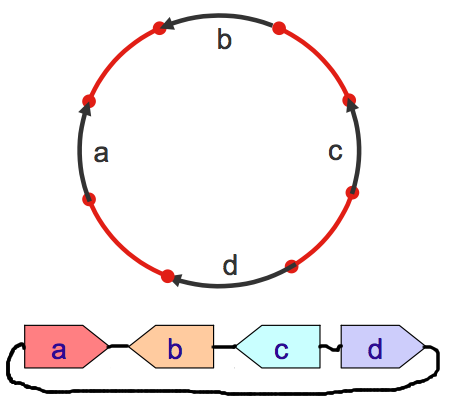
\includegraphics[max width=0.5\linewidth]{fig/1/block_graph.png}
  \caption{Граф блоков циклической хромосомы}
  \label{fig:block_graph}
\end{figure}
Рассмотрим одиночную циклическую хромосому, разбитую на уникальные блоки синтении.
Хромосома в виде перестановки над блоками синтении может быть представлена как граф с двумя типами ребер:
направленными, обозначающими блоки синтении, и ненаправленными, обозначающими связи между блоками.
В таком представлении для блока $a$ назовем вершину в которую входит обозначающее его ребро $a_h$, а вершину из которой это ребро исходит - $a_t$.
После такого переименования можно заметить, что даже при удалении направленных ребер информация о них не потеряется.
Таким образом, можно перейти к представлению графа в виде списка смежности вершин,
где вершины считаются смежными, если они соединены ненаправленным ребром.
Например, на рисунке~\ref{fig:block_graph} граф может быть представлен в виде списка ребер $[(a_h, b_h)$, $(b_t, c_h)$, $(c_t, d_t)$, $(d_h, a_t)]$,
из которого исходный граф может быть восстановлен.
Описанное выше представление не дает возможности работать с линейными хромосомами,
первый и последний синтенные блоки которых связаны с предыдущим и следующим за ними синтенным блоком соответственно, потому
данное представление можно обобщить, добавив специальную фиктивную вершину $\infty$,
с которой будут связаны первый и последний синтенные блоки в хромосоме~\cite{Alekseyev2009}.
Далее определим, что для объединения двух хромосом список смежности получается объединением списков смежностей для каждой из них.
Используя описание выше, становится возможным превратить биологический объект (набор хромосом) в математический объект (граф смежностей),
далее будет рассмотрено как нас основе геномов в таком виде возможно оценивать расстояния между ними.

Теперь перейдем к рассмотрению нескольких геномов.
Для начала примем, что геномы определены на одних и тех же блоках синтении и в каждом из геномов они все присутствуют в единичном экземпляре.
Для описания графового представления сразу нескольких геномов нам понадобится понятие \textit{индексированного объединения}.
\begin{define}{Индексированное объединение} \\
  Пусть имеется два множества $A$ и $B$ и множество индексов $\bb{I}$, тогда их индексированное объединение
  $A \cup_{\bb{I}} B$ имеет вид $\{ (i, a) | \forall a \in A, i \in \bb{I}\} \cup \{ (j, b) | \forall b \in B, j \in \bb{I}\}, i \neq j$.
\end{define}
Для объединения геномов вышеописанная структура графа определяется как индексированное объединение списков смежности, где индексами является множество цветов.
Так как в данном представлении каждый геном имеет свой уникальный цвет, в дальнейшем слова \q{геном} и \q{цвет} будут использоваться взаимозаменяемо.
Смысл предыдущей операции состоит в том, чтобы объединить графы смежности для обоих геномов не теряя информации, к какому геному какое ребро принадлежит.
Структура графа выше имеет название \q{брейкпоинт граф}~\cite{bafna1996genome}.
\begin{figure}[H]
  \centering
  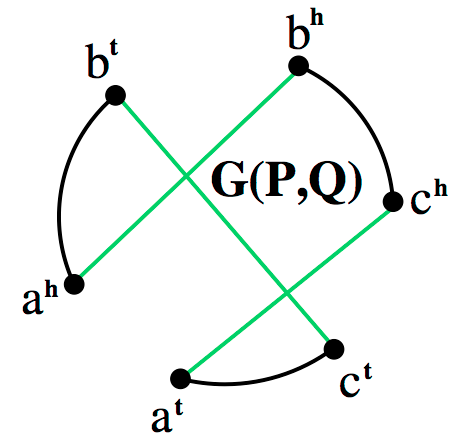
\includegraphics[max width=0.4\linewidth]{fig/1/two_genomes_bp_graph.png}
  \caption{Брейкпоинт граф для пары геномов со списками ребер $[(a_h, b_t), (b_h, c_h), (c_t, a_t)]$ и $[(a_h, b_h), (b_t, c_t), (c_h, a_h)]$.}
  \label{fig:two_genomes_bp_graph}
\end{figure}
Пример брейкпоинт графа для пары геномов приведен на рисунке~\ref{fig:two_genomes_bp_graph}.
Представление геномов в виде брейкпоинт графа позволяет сосредоточиться рассмотрении связей между синтенными блоками
и применять для этого существующие методы работы с графами.
Также можно определить такую структуру для количества геномов больше двух:
для этого для каждого следующего генома выбирается новый цвет и его ребра добавляются к имеющимся.
Брейкпоинт граф для множества геномов также называется \q{множественный брейкпоинт граф}~\cite{caprara1999tightness}.
Таким образом, получается структура, хранящая в себе информацию о смежностях блоков сразу во многих геномах определенных на этих блоках.
Полученный множественный брейкпоинт граф для $N$ геномов при условии, что каждый из геномов определен на одном и том же множестве синтенных блоков
будет $N$-регулярным, вставка или удаление блоков в какие-либо из геномов приведет к тому, что $N$-регулярность потеряется,
но в остальном не изменит устройства графа.

Имея брейкпоинт граф для геномов становится возможным ввести оценку филогенетического расстояния между ними.
Для этого введем операцию выполняемую над брейкпоинт графом, называемую 2-брейк.
\begin{figure}[H]
  \centering
  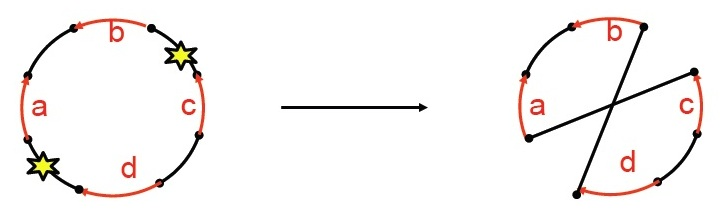
\includegraphics[max width=0.5\linewidth]{fig/1/2break.jpg}
  \caption{2-брейк}
  \label{fig:2break}
\end{figure}
\begin{define}{2-брейк (Double Cut and Join, DCJ)}~\cite{bergeron2006unifying} \\
  Назовем 2-брейком следующую операцию: удаление 2 ребер в брейкпоинт графе и добавление новых двух ребер на ``освободившихся'' вершинах
  несовпадающих с удаленными (рисунок~\ref{fig:2break}).
\end{define}
При выполнении 2-брейка над брейкпоинт графом количество компонент связности в нем может уменьшиться или увеличиться.
Когда количество компонент связности в брейкпоинт графе достигнет максимума (граф разобьется на циклы длины 2),
для двух геномов это будет обозначать, что они трансформировались в один, то есть пришли к состоянию генома их общего предка.
Так как последовательность 2-брейков, которая приведет к такому состоянию графа может быть любой длины, если выбрать кратчайшую такую последовательность,
то ее длина будет равна оценке эволюционного расстояния между геномами при условии того, что в процессе эволюции происходили только 2-брейки.
\begin{define}{2-брейк расстояние (DCJ-расстояние, $d_{DCJ}$)} \\
  2-брейк расстояние - длина кратчайшей последовательности из 2-брейков приводящей
  исходный брейкпоинт граф в состояние с наибольшим числом компонент связности.
\end{define}

Данное расстояние может быть расширено для учета различных структурных изменений строения молекулы ДНК~\cite{yancopoulos2009dcj}.
На практике также используется оценка расстояния, называемая брейкпоинт расстояние~\cite{blanchette1997breakpoint}.

\begin{define}{Брейкпоинт расстояние (BP-расстояние, $d_{BP}$)} \\
  Брейкпоинт расстояние - расстояние, вычисляемое по формуле $d_{BP} = n - a - \frac{t}{2}$,
  где $n$ - количество генов в каждом геноме,
  $a$ - количество общих связностей для двух геномов, $t$ - количество
  общих связностей, где один конец связности является вершиной $\infty$.
\end{define}
Метрика брейкпоинт расстояния наиболее простая в вычислении и не требует выбора модели эволюции
(определения, какие операции могли происходить в процессе эволюции)~\cite{blanchette1997breakpoint}.

Используя введенные определения расстояний можно перейти к обзору существующих инструментов,
решающих поставленную выше проблему.

\section{Существующие решения}

В решении задачи восстановления филогенетических деревьев есть три основных подхода:
\begin{enumerate}
  \item На основе матрицы расстояний (Distance Methods, DM)
  \item Максимального правдоподобия (Maximum Likelihood, ML)
  \item Максимальной бережливости (Maximum Parsimony, MP)
\end{enumerate}

Далее рассматриваются инструменты представляющие все три подхода.

\subsection{TreeInferer (Ragout) и TIBA~\cite{lin2012tiba}}
Оба инструмента восстанавливают деревья с на основе матрицы расстояний.
Восстановление деревьев в данном подходе делится на две части:
поиск попарных расстояний между геномами и восстановление дерева из матрицы известных расстояний
(с возможным пересчетом матрицы на каждом шаге).
И подсчет расстояний и восстановление дерева в данном подходе может осуществляться с использованием различных оценок, что дает подходу гибкость.
TreeInferer, будучи частью сборщика Ragout~\cite{Kolmogorov2014}, может работать с несобранными данными
и использует $d_{BP}$ в связке с Neighbour Joining~\cite{saitou1987neighbor}.
TIBA работает только с собранными геномами, использует оценку $d_{DCJ}$
и либо Neighbour Joining, либо еще один механизм восстановления деревьев на основе матрицы расстояний, FastME~\cite{desper2002fast}.
Стоит отметить, что оба этих инструмента работают только на геномах без вставок и удалений блоков
и не могут учитывать информацию об известных поддеревьях.

\subsection{MLWD~\cite{hu2014mlgo}}
Данный инструмент использует подход максимального правдоподобия.
В данном подходе ключевым моментом является выбор вероятностной модели - математической модели,
которая позволяет оценить правдоподобие филогенетического дерева при условии имеющихся листовых геномов
и далее выбрать то дерево, что имеет наибольшее правдоподобие.
Данный подход делает инструменты с ее использованием труднорасширяемыми,
но взамен позволяет строить модели более точно отражающие эволюционные процессы происходящие в действительности.
MLWD использует данное преимущество и потому поддерживает работу с блоками, полученными из несобранных геномов,
с вставками, удалениями и дупликациями генов, но также как
и прошлые инструменты не может использовать информацию об известных поддеревьях.

\subsection{GAS Phylogeny}
Этот инструмент использует подход максимальной бережливости.
Суть данного подхода состоит в построении модели,
в которой каждое эволюционное событие имеет вклад в оценку восстановленного дерева, и дальнейшего нахождения дерева с наименьшей такой оценкой.
Можно сказать, что метод максимального правдоподобия это частный случай метода максимальной бережливости, когда функция оценки является
еще и вероятностью получить то или иное дерево в поставленной модели.
Задача поиска филогенетического дерева с наименьшей оценкой принадлежит к классу NP-трудных, потому зачастую при использовании данного подхода
применяются эвристические оценки вместо точных и выбирается возможно неоптимальное, но, тем не менее, имеющее близкую к оптимальной оценку.
В представленном инструменте~\cite{xu2011gasts} используется эвристическая оценка $S_{GASTS}$, позволяющая ему работать быстро и при этом выдавать точный результат.
Данный инструмент не умеет обрабатывать данные, полученные из несобранных геномов, имеющих вставки или удаления и не учитывает информацию об
известных поддеревьях.

\section{Филогенетическая информация в брейкпоинт графе}

Опишем основания для выбора предлагаемого в данной работе подхода.
Рассмотрим теперь множественный брейкпоинт граф для геномов и некое неизвестное филогенетическое дерево для них.
В процессе эволюции геном потомка получается из генома предка с помощью структурных и точечных изменений.
Теперь если рассмотреть брейкпоинт граф полученный из генома потомка,
то выполняя на нем операции 2-брейков обратные произошедшим можно получить из него геном предка~\cite{Alekseyev2009}.
Имея же брейкпоинт граф, построенный на основе геномов нескольких потомков,
можно выполняя 2-брейки на ребрах разных цветов получать из геномов потомков геномы их общих предков,
а разные последовательности выполненных 2-брейков будут задавать разные филогенетические деревья на геномах потомков.
% В процессе эволюции молекула ДНК подвергалась структурным изменениям при движении от корня филогенетического дерева к листьям.
% Имея же на руках брейкпоинт граф для листовых геномов можно сопоставить операции на нем с поворачиванием вспять истории структурных изменений,
% иначе говоря, движением по филогенетическому дереву от листьев к корню:
% при выполнении операций 2-брейк, приводящих к увеличению компонент связности, происходит, по сути, обращение структурных изменений,
% произошедших на ветвях дерева в процессе эволюции.
Таким образом, в брейкпоинт графе \q{закодирована} информация о филогенетическом дереве в виде преобразований над корневым геномом,
ребра различных цветов же, содержат такую информацию для каждого из потомков.
Данная информация может быть представлена, например, как требование того, что геномы потомков лежат в разных поддеревьях филогенетического дерева.

Теперь можно описать главную проблему, решаемую в данной работе.

\section{Задача восстановления деревьев}
Главной проблемой в данной работе является проблема восстановления филогенетических деревьев из брейкпоинт графа.
На пути к ее решению ставятся две задачи:
\begin{enumerate}
  \item Найти способы извлечения информации из брейкпоинт графа
  \item Найти способы из извлеченной информации построить филогенетическое дерево
\end{enumerate}

% Глава 2
\chapter{Восстановление филогенетических деревьев из брейкпоинт графа}

\section{Получение информации из брейкпоинт графа}
Описанные в предыдущей главе методы вычисления редакционного расстояния между геномами можно рассмотреть в ином ключе.
Редакционное расстояние в модели методов основанных на расстояниях \q{стягивает} геномы друг к другу, заставляя их находиться ближе в дереве, то есть,
принимается, что геномы с меньшим редакционным расстоянием находятся в одном поддереве с большей вероятностью.
Иными словами, расстояние дает нам филогенетическую информацию о ветвях в филогенетическом дереве.

В~\cite{xu2010exploring} автор рассматривает несколько оценок редакционного расстояния, включая описанные выше
и вводит концепцию филогенетического паттерна позволяющую применять их к восстановлению деревьев из брейкпоинт графа.
\begin{define}{Филогенетический паттерн} \\
  Филогенетический паттерн $P(\bb{G}, T)$, где $\bb{G}$ - множество геномов,
  а $T$ - топология филогенетического дерева на них - функция, которая для данных входных геномов
  сопоставляет каждой из возможных топологий филогенетического дерева эвристическую оценку так,
  чтобы она была экстремальной только на одной топологии.
\end{define}
Главное свойство данной концепции в том, что имея на руках листовые геномы филогенетического дерева, можно получить всегда только одно возможное дерево.
Тогда если найти филогенетический паттерн, который будет давать экстремальное значение на тех же топологиях,
что и другая оценка $s$ (например, $d_{BP}$), то он будет давать ту же филогенетическую информацию, что и $s$, несмотря на то,
что эту оценку невозможно было бы вычислить, не зная предковых геномов.
Получается, что имея на руках паттерн, то становится возможным получать оптимальное дерево с точки зрения использованной оценки.
Более того, возможно определить множество паттернов, каждый из которых, в общем случае, может давать экстремальное значение на разных топологиях,
для этого для каждого из паттернов необходимо определить тот вес, который он вносит в оценку, для каждого паттерна это будет рассмотрено отдельно.
В~\cite{xu2010exploring} показано, что филогенетические паттерны удобно строить на основе подграфов брейкпоинт графа,
так как зачастую информации (значений оценки) получаемой на основе малых подграфов достаточно для того,
чтобы отличить разные топологии филогенетического дерева и восстановить корректное.
В дальнейшем филогенетический паттерн и подграф на котором он вычисляется будут использоваться взаимозаменяемо.
Рассмотрим предложенный в~\cite{xu2010exploring} паттерн \q{контрастирующая смежность}.
\begin{figure}[H]
  \centering
  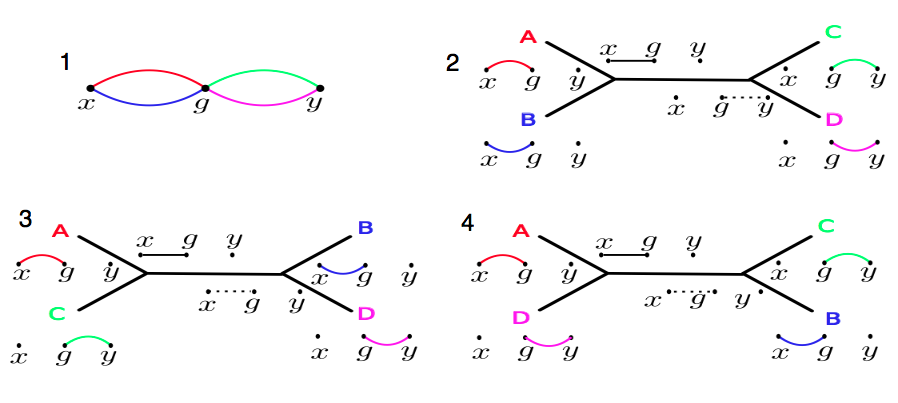
\includegraphics[max width=\linewidth]{fig/2/contrasting_adjacency.png}
  \caption{Контрастирующая смежность.
    1 - подграф, на котором базируется паттерн;
    2 - дерево с топологией $AB|CD$, на котором достигается экстремальное значение $d_{DCJ}$ и $d_{BP}$;
    3, 4 - другие возможные топологии, на которых не достигается экстремальное значение метрик $d_{DCJ}$ и $d_{BP}$}
  \label{fig:contrasting_adjacency}
\end{figure}
Этот паттерн представляет собой подграф брейкпоинт графа из трех вершин, где одна пара соединена двумя ребрами цветов $A$ и $B$, а другая - $C$ и $D$.
Обозначим, что для 4 геномов $A, B, C, D$, $AB|CD$ обозначает, что геномы $A$ и $B$ находятся в одном поддереве, а $C$ и $D$ - в другом.
Тогда для топологии $AB|CD$ можно посчитать расстояние $d (d_{DCJ}, d_{BP})$ как $d(A, B) + d(C, D) + d(I_1, I_2)$,
где $d(\_, \_)$ - функция расстояния между двумя геномами, $I_1, I_2$ - предки в дереве на парах геномов $AB$ и $CD$ соответственно.
Из рисунка~\ref{fig:contrasting_adjacency} можно увидеть, что на топологии $AB|CD$ оценки $d_{BP}$ и $d_{DCJ}$, полученные как указано выше, достигают минимального значения.
Вышеописанный паттерн был обобщен для многих геномов в~\cite{Alekseyev2009} с помощью концепции \textit{простого пути}.
Для того, чтобы ввести эту концепцию введем понятие \textit{альтернирующих мультицветов} на последовательности ребер.
\begin{define}{Альтернирующие мультицвета} \\
  Альтернирующие мультицвета на последовательности ребер $\{e_i\}$ - пара мультицветов $Q$ и $Q'$, таких что
  $\forall i$ если цвет $e_i$ $Q$, то цвет $e_{i + 1}$ - $Q'$ и наоборот, если цвет $e_i$ $Q'$, то цвет $e_{i + 1}$ - $Q$.
\end{define}

\begin{define}{Простой путь} \\
  Простой путь - путь в брейкпоинт графе, состоящий из вершин мультистепени 2 и ребер двух
  мультицветов $Q$ и $Q'$, таких что $Q \cap Q' = \varnothing \land Q \cup Q' = \bb{Q}$,
  где $\bb{Q}$ - множество всех цветов, если путь состоит из последовательности ребер $\{e_i\}$,
  то цвета $Q$ и $Q'$ альтернирующие на $\{e_i\}$.
\end{define}
Оба этих паттерна дают более экстремальную оценку для тех деревьев,
в которых геномы из каждого из альтернирующих мультицветов находятся в одном поддереве.

В брейкпоинт графе один и тот же филогенетический паттерн может встречаться несколько раз и
\q{свидетельствовать} о разном строении филогенетического дерева (более экстремальная оценка достигается на деревьях с разной топологией),
это происходит из-за того, что в паттерн включается только подграф брейкпоинт графа.
Основываясь на предыдущем замечании, можно понять, что информация (\q{свидетельства} о расположении геномов в поддеревьях филогенетического дерева)
извлеченная из брейкпоинт графа будет тем точнее,
чем больше непересекающихся (не использующих одни и те же основания для различия топологий) паттернов будет найдено.
Так становится необходимым искать непересекающиеся филогенетические паттерны в брейкпоинт графах.

Определение паттернов вручную - тяжелый и медленный процесс, потому в данной работе предложен метод их автоматического поиска.
Филогенетический паттерн - это подграф в брейкпоинт графе, раскрашенный в несколько цветов.
Важно заметить два факта:
\begin{enumerate}
  \item Каждый цвет в данном случае необязательно соответствует одному геному, но может соответствовать целой их группе.
  \item Если взять ребра одного цвета из подграфа образующего филогенетический паттерн, то они не будут вершинно пересекаться и образуют паросочетание.
\end{enumerate}

Первый факт важен для получения информации с помощью филогенетических паттернов из брейкпоинт графов для многих геномов,
а второй позволяет перейти к автоматическому поиску филогенетических паттернов.
\begin{figure}[H]
  \centering
  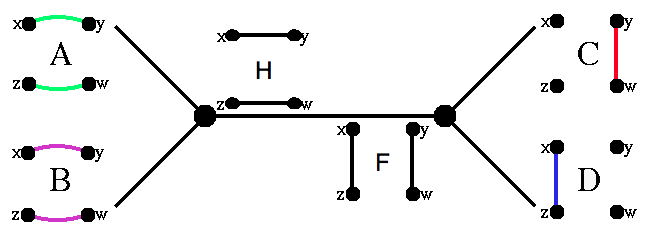
\includegraphics[max width=0.5\linewidth]{fig/2/automatic_pattern_search.png}
  \caption{Схема для перебора паттернов.
    $A, B, C, D$ - конфигурации листовых геномов, каждый из которых является паросочетанием на вершинах брейкпоинт графа.
    $H, F$ - предковые геномы, каждый из которых также является паросочетанием.}
  \label{fig:automatic_pattern_search}
\end{figure}
На рисунке~\ref{fig:automatic_pattern_search} показана схема для перебора паттернов.
Целью перебора является поиск таких 4 конфигураций геномов, на которых обе оценки ($d_{BP}$, $d_{DCJ}$) или одна из них
достигает экстремального значения на одной топологии дерева, но не достигает его на других.
Условие выше выполняется если найдется такая пара конфигураций внутренних вершин,
что на одной из топологий достигается более экстремальное значение оценки, когда на других оно не достигается,
что говорит о том, что найденный набор конфигураций есть филогенетический паттерн.
Ниже представлен алгоритм поиска:
\begin{enumerate}
  \item Выбрать с повторениями 4 паросочетания, как конфигурации геномов.
  \item Для каждой из 3 топологий перебрать паросочетания для внутренних вершин (они тоже являются паросочетаниями).
  \item Выбрать те кортежи из 4 геномов, на которых оценка достигает экстремума.
\end{enumerate}

Важно заметить, что алгоритм выше выполняет перебор, без проверки на уникальность найденных графов, потому необходимо удалить \q{похожие} из них.
Для этого можно определить понятие \textit{изоморфизма паттернов}.
\begin{define}{Изоморфизм паттернов} \\
  Паттерны $A$ и $B$ изоморфны тогда и только тогда, когда существует пара биективных отображений $(f, h)$,
  $f$ - между вершинами паттерна $A$ вершинами паттерна $B$, $h$ - между ребрами паттерна $A$ и ребрами паттерна $B$,
  такая что любые две вершины $u$ и $v$ в $A$ связаны мультимножеством раскрашенных ребер $E$ тогда и только тогда, когда вершины
  $f(u)$ и $f(v)$ связаны $h(E)$.
\end{define}
\vspace{-2em}
\begin{figure}[H]
  \centering
  \minipage{0.25\textwidth}
  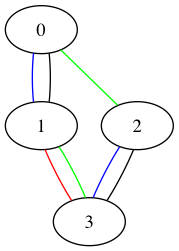
\includegraphics[max width=\linewidth]{fig/2/patterns/similar1.png}
  \endminipage
  \minipage{0.25\textwidth}
    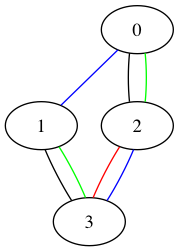
\includegraphics[max width=\linewidth]{fig/2/patterns/similar2.png}
  \endminipage
  \caption{Изоморфные паттерны}
  \label{fig:isomorphic_patterns}
\end{figure}

Таким образом, могут быть найдены все паттерны на любом количестве вершин.
В данной работе удалось провести поиск паттернов на 4 вершинах (перебор на большем числе вершин оказался слишком вычислительно затратным),
в результате него после отсеивания изоморфных паттернов и паттернов, которые учитывались бы в оценках, используемых Wei Xu
(паттерны, содержащие простые пути длины больше 1 или простые циклы) остались следующие паттерны,
показанные на рисунках~\ref{fig:cylinder_pattern} и~\ref{fig:bag_pattern}.
Оба этих паттерна дают более экстремальную оценку для деревьев, в которых цвета,
из которых состоят ребра помеченные звездочкой, находятся в одном поддереве.
\begin{figure}[H]
  \centering
  \minipage{0.25\textwidth}
  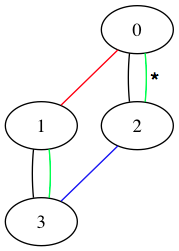
\includegraphics[max width=\linewidth]{fig/2/patterns/cylinder.png}
    \caption{Паттерн \q{цилиндр}}
    \label{fig:cylinder_pattern}
  \endminipage \hspace{1em}
  \minipage{0.25\textwidth}
  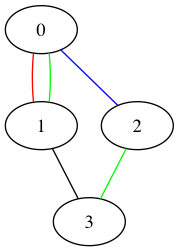
\includegraphics[max width=\linewidth]{fig/2/patterns/bag.png}
    \caption{Паттерн \q{мешок}}
    \label{fig:bag_pattern}
  \endminipage
\end{figure}

\section{Сборка деревьев из разделений}
Смысл использования филогенетических паттернов для восстановления деревьев заключается в том,
чтобы извлечь информацию о устройстве филогенетического дерева из брейкпоинт графа в удобном для восстановления виде.
Так каждая копия филогенетического паттерна найденная в брейкпоинт графе дает информацию о том,
что одна часть геномов находятся ближе друг к другу, а другие - дальше друг от друга в филогенетическом дереве.
Например, если в графе встречается паттерн \q{простой путь} на двух альтернирующих цветах $Q$ и $Q'$, то он \q{свидетельствует},
что геномы из множества $Q$ находятся в одном поддереве, а геномы из множества $Q'$ - в другом, как показано на рисунке~\ref{fig:division}.
\begin{figure}[H]
  \centering
  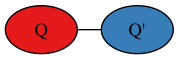
\includegraphics[max width=0.5\linewidth]{fig/2/division.png}
  \caption{Дерево, о котором \q{свидетельствует} простой путь на альтернирующих цветах $Q$ и $Q'$.}
  \label{fig:division}
\end{figure}
Таким образом, механизм филогенетических паттернов позволяет получить из брейкпоинт графа информацию о ветвях филогенетического дерева.
Сформулируем задачу восстановления филогенетического дерева из полученной информации.
Для этого введем понятие \textit{разделения} как единицы информации об устройстве филогенетического дерева.
\begin{define}{Разделение} \\
  Пусть $\bb{Q}$ - множество всех листовых геномов.
  Разделение - пара множеств вида $Q_1|Q_2$, таких, что $Q_1 \subset \bb{Q}$ и $Q_2 \subset \bb{Q}$ и при этом
  $Q_1 \cap Q_2 = \varnothing$ и $Q_1 \cup Q_2 = \bb{Q}$.
\end{define}
Введем обозначения что для разделения вида $D = Q_1|Q_2$, $left(D) = Q_1$, $right(D) = Q_2$.
Также заметим, что для дальнейшего использования разделения $Q_1|Q_2$ и $Q_2|Q_1$,
где $Q_1$, $Q_2$ - подмножества множества всех геномов $\bb{Q}$, идентичны.

Представим каждое вхождение паттерна $P$ в брейкпоинт граф как разделение $Q_1|Q_2$,
если согласно вхождению паттерна $P$ геномы $Q_1$ должны находиться в одном поддереве результирующего филогенетического дерева,
а геномы $Q_2$ - в другом.
Таким образом, если $search(G, P)$ дает набор всех вхождений паттерна $P$ в брейкпоинт граф $G$,
а $toDivision_P(I)$ преобразует вхождение $I$ паттерна $P$ в разделение,
то набор разделений $\bb{D}$ полученный из брейкпоинт графа $G$ и множества паттернов $\bb{P}$ можно выразить как
$\bigcup\nolimits_{P \in \bb{P}} \bigcup\nolimits_{I \in search(G, P)} \{toDivision_P(I)\}$.
В таком случае все разделения считаются одинаково ценными и неясно, как восстановить дерево из них, так как непонятно,
как выбирать из двух противоречащих друг другу разделений то, которое должно войти в результирующее дерево,
потому введем понятие \textit{свидетельства}.
\begin{define}{Свидетельство}\\
  Свидетельство - пара разделения и оценки, указывающей, насколько весома информация о наличии данного разделения в результирующем филогенетического дерева.
\end{define}
Например, простой путь длины $l$ на альтернирующих цветах $Q$ и $Q'$ дает свидетельство в $\floor{\frac{l}{2}}$ единиц и
свидетельство ($Q|Q'$, $\floor{\frac{l}{2}}$).
Далее, сгруппируем все свидетельства с одинаковыми разделениями и сложим их оценки.
Тогда мы получим множество свидетельств $\bb{S} = \{(D, V)\}$, где каждое разделение $D$ встречается не больше одного раза.
Обозначим, что для свидетельства $S = (D, V)$, $D = div(S)$ и $V = value(S)$, а $left(S) = left(div(S))$ и $right(S) = right(div(S))$.
Сформулируем теперь задачу, решение которой даст нам лучшее восстановленное дерево из возможных на основе выделенной филогенетической информации.
\begin{task}{Восстановление филогенетического дерева из свидетельств} \\
  Восстановить филогенетическое дерево с наилучшей оценкой имея на входе набор свидетельств,
  полученных из брейкпоинт графа.
\end{task}

В данной работе будет описано два алгоритма восстановления деревьев из полученных свидетельств:
наивный алгоритм и реализация динамическим программированием.
Для описания алгоритмов введем отношение \textit{непересечения} между двумя разделениями.
\begin{define}{Непересекающиеся разделения} \\
  Два разделения $Q_1|Q_2$ и $R_1|R_2$ \textit{не пересекаются},
  если $Q_1 \cap R_1 = \varnothing \lor Q_1 \cap R_2 = \varnothing $.
\end{define}
\noindent Отношение непересечения симметрично.

\subsection{Наивный алгоритм}
Суть данного алгоритма в том, чтобы перебрать все деревья, о которых \q{свидетельствует} брейкпоинт граф и выбрать из них лучшее.
Отличие данного алгоритма от полного перебора всех деревьев с их оцениванием в том,
что основываясь на свидетельствах полученных из имеющегося брейкпоинт графа часть из них построить невозможно, а поэтому
перебор уменьшится.
Введем понятие \textit{класса непересекающихся разделений}, которое описывает возможное дерево в виде разделений.
\begin{define}{Класс непересекающихся разделений} \\
  Класс непересекающихся разделений $F$ над множеством разделений $\bb{D}$ - подмножество $\bb{D}$,
  в котором любые два разделения не пересекаются между собой.
\end{define}

\noindent Таким же образом определим понятие \textit{класса непересекающихся свидетельств}.
\begin{define}{Класс непересекающихся свидетельств}\\
  Класс непересекающихся свидетельств $H$ над множеством свидетельств $\bb{S}$ - подмножество $\bb{S}$,
  такое что $\forall S \in H: div(S) \in F$,
  где $F$ -  класс непересекающихся разделений над множеством разделений.
\end{define}

\noindent Для класса непересекающихся свидетельств $H$ определим его оценку \\
$value(H) = \sum\nolimits_{S \in H} value(S)$.

\begin{define}{Максимальный класс непересекающихся разделений} \\
  Максимальный класс непересекающихся разделений $F$ на множеством разделений $\bb{D}$ -
  класс непересекающихся разделений над $\bb{D}$, такой что него невозможно добавить новое разделение из $\bb{D}$,
  так чтобы он сохранил свойство непересечения.
\end{define}

\begin{define}{Максимальный класс непересекающихся свидетельств} \\
  Максимальный класс непересекающихся свидетельств $H$ над множеством свидетельств $\bb{S}$ - класс непересекающихся свидетельств $H$,
  такой что $\forall S \in H: div(S) \in F$,
  где $F$ - максимальный класс непересекающихся разделений над множеством разделений.
\end{define}

Заметим, что из исходного множества разделений, в общем случае, можно получить несколько максимальных классов непересекающихся разделений.
\begin{example}
  Рассмотрим случай, что $\bb{D} = \{ AB|CD, AC|BD, A|BCD \}$, где $A, B, C, D$ - геномы.
  В данном случае можно получить максимальные классы непересекающихся разделений
  $H_0 = \{ AB|CD, A|BCD \}$ и $H_1 = \{ AC|BD, A|BCD \}$.
\end{example}
Из этого примера также видно, что разделение может входить в несколько непересекающихся классов разделений одновременно,
что соответствует тому случаю, когда одна ветвь присутствует в разных деревьях.
В~\cite{gusfield1991efficient} показано, что из класса непересекающихся разделений можно построить дерево единственным образом:
для этого необходимо выписать разделения в таблицу $M \times N$, где $M$ - количество разделений в классе, $N$ - количество геномов,
и для каждого генома $G$ и разделения $D = Q_1|Q_2$ записать на их пересечении 1, если $G \in Q_1$ и ноль иначе.

На основе вышеизложенного сформулируем наивный алгоритм:
\begin{enumerate}
  \item Выделить среди свидетельств множество максимальных классов непересекающихся $\bb{C}$
  \item Выбрать лучший по оценке класс из $\bb{C}$
  \item Выделить разделения из свидетельств выбранного класса и собрать из них дерево
\end{enumerate}

\subsection{Реализация динамическим программированием}

Проблемой предыдущего алгоритма являлось то, что он выполнял перебор всех деревьев, о которых \q{свидетельствует} брейкпоинт граф,
в случае многих геномов таких деревьев может быть много, что приведет к тому, что работа алгоритма может занять большое время.
Каждое разделение вида $Q_1|Q_2$ задает ветку в некорневом бинарном дереве с помеченными листьями, иными словами,
делит все множество геномов на два подмножества $Q_1$ и $Q_2$, топология дерева на которых
(расположение геномов из подмножества в филогенетическом дереве) может быть уточнена в дальнейшем другими разделениями.
Из этого следует, что поиск топологий для подмножеств может проводится независимо.
Поиск топологий на подмножестве геномов $G'$ - такая же задача как исходная, но при этом для каждого разделения $D$
из множества разделений (и каждого свидетельства с разделением $D$) из $D$ удаляются все геномы, не присутствующие в $G'$
Теперь, если для любого свидетельства $S$ с разделением вида $Q_1|Q_2$ из некоторого набора $\bb{S}$ известны топологии с наилучшей оценкой,
построенные на множествах геномов $Q_1$ и $Q_2$, то чтобы найти дерево с максимальной оценкой нужно перебрать все свидетельства из $\bb{S}$ и найти то,
оценка которого в сумме с оценками поддеревьев даст наибольшее значение.
Данную логику можно применить также для того, чтобы построить оптимальные деревья для вышеупомянутых пар множеств $Q_1$ и $Q_2$,
составляющих разделения свидетельств.
Таким образом, приходим к задаче динамического программирования для решения которой сформулируем следующий алгоритм:
\begin{enumerate}
  \item Обозначим, что для любого множества $F$ размера $f$, $size(F) = f$.
    Пусть даны множества $\bb{G}$ геномов и $\bb{S}$ имеющихся свидетельств.
    Выпишем построчно набор множеств $\{ SCLevel_i | i = 1..N \}$ в порядке убывания $i$, где $N = size(\bb{G})$,
    a $\forall i, SCLevel_i$ - множество четверок вида $(C, V, V, (null, null))$, таких что $size(C) = i$,
    $\exists S \in \bb{S}: (C = left(S) \lor C = right(S)) \land value(S) = V$ ($null$ обозначает отсутствие значения).
    Компоненты четверки обозначают соответственно: множество геномов, для которого известна топология филогенетического дерева;
    оценку этого множества (оценку свидетельства, в разделении которого это множество присутствует);
    суммарную оценку построенного дерева; пару множеств геномов, на которые делится данное множество геномов.
  \item Начиная с $i = 2$,
    $\forall c = (C, V, CS, SS) \in SCLevel_i$,
    $(C1, V1, CS1, SS1) \in SCLevel_j$,
    $(C2, V2, CS2, SS2) \in SCLevel_k$ обозначим, что $c = (C, V, V + CS1 + CS2, (C1, C2))$,
    если $V + CS1 + CS2$ - максимальное значение при условии  $j = 1..i-1$, $k = i - j$ и $C1 \cup C2 = C \land C1 \cap C2 = \varnothing$
  \item Пусть единственный элемент $SCLevel_N$ имеет вид $(C, V, CS, (C1, C2))$ тогда результирующее дерево можно построить сверху
    вниз для множеств $C1$ и $C2$, после чего объединить результаты корнем.
    Для множеств $C1$ и $C2$ можно выполнить сборку тем же образом, базой для индукции послужит случай,
    когда $C1$ и $C2$ - множества с одним элементом.
\end{enumerate}

\subsection{Примечания к практической реализации}

В первой главе были описаны недостатки существующих решений, которые не позволяли бы им работать с блоками, полученными из геномов со вставками
и удалениями, несобранными геномами или использовать для восстановления информацию об известных поддеревьях восстанавливаемого дерева.
Опишем, как предложенный подход борется с данными проблемами.

Рассмотрим, что происходит с брейкпоинт графом при работе с данными в которых происходили вставки или удаления блоков,
рассмотрим только случай циклических хромосом (в линейных различия будут случаться только в конечных блоках):
при удалении или вставке блока 2 вершины брейкпоинт графа теряют степень $N$ ($N$ - количество геномов), при вставке степень растет,
при удалении - падает.
Для того, чтобы \q{не потерять} структуры графа, зависящие от данных вершин в случае удаления блока выполняется добавление \q{протезного} ребра
необходимого цвета.
Далее свидетельства на графе считаются так же как и раньше, но к результирующим свидетельствам добавляется информация (в форме оценки) о том,
что было добавлено ребро такого цвета.
Данные преобразования приводят к тому, что даже в условиях большого количества вставок или удалений в графе все равно возможно найти
структуры, которые исчезли в процессе эволюции, но при этом также не теряется информация о том, что вставки или удаления произошли.

При работе с несобранными данными возникает проблема того, что при разбиении хромосомы собранного генома теряется одна смежность на каждые
два контига.
Данная потеря не наносит большого вреда, так как обычно при работе с несобранными геномами блоков много больше (зачастую на несколько порядков),
чем контигов, таким образом, потеря связностей из-за несобранности геномов мало влияет на процесс восстановления деревьев.

При работе с реальными данными, возможна ситуация когда из биологических источников доступна информация о расположении геномов в филогенетическом дереве.
Для того, чтобы поддержать работу с известными поддеревьями используется идея того, что любое разделение из известного поддерева должно присутствовать в результирующем.
Для того, чтобы обеспечить выполнение этого требования известное поддерево разбивается на разделения следующим образом:
\begin{enumerate}
  \item Пусть есть известное поддерево $(T, Q) = ((T_1, Q_1), (T_2, Q_2))$, где $T, T_1, T_2$ - бинарные деревья,
    а $Q, Q_1, Q_2$ - множества геномов в содержащиеся, $\bb{Q}$ - множество всех геномов,
    тогда для такого дерева набор разделений $Divisions(T)$ будет выглядеть как
    $\{Q|\bb{Q} \setminus  Q,$ $Q_1|\bb{Q} \setminus Q_1,$ $Q_2|\bb{Q} \setminus Q_2\} \cup Divisions(T_1) \cup Divisions(T_2)$,
    базой для данной индукции будет случай, когда $Q$ - множество из одного генома.
  \item Для каждого из полученных разделений назначаем оценку $\bb{V}=$ \\
    $\sum\nolimits_{S \in \bb{S}} value(S)$, где $\bb{S}$ - множество свидетельств, полученных из брейкпоинт графа.
\end{enumerate}
После таких операций каждое разделение из известного поддерева окажется в результате, так как при сборке любое пересекающееся с ним разделение
принесет меньше веса в оценку результирующего дерева и потому не будет взято.

% Глава 2
\chapter{Тестирование}
Тестирование результатов выполнялось в два этапа: тестирование найденных филогенетических паттернов и тестирование
восстановления деревьев с помощью MGRA2.

\section{Тестирование найденных паттернов}
В тестировании на симуляционных данных используется консервативная проверка правильности восстановления -
если восстановленное дерево не совпадает с верным (RF-метрика~\cite{Robinson1981} не дает расстояние 0)
или, в случае тестирования паттернов, другое дерево из возможных имеет ту же оценку, то дерево считается неправильно восстановленным.

\subsection{Тестирование на геномах со случайными брейкпоинт графами}
Для тестирования найденных паттернов использовался подход описанный в~\cite{xu2010exploring}.
Генерировались случайные геномы, состоящие из одной циклической хромосомы с 200 генами.
\begin{figure}[H]
  \centering
  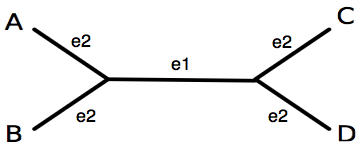
\includegraphics[max width=0.5\textwidth]{fig/3/wei_xu_tree.png}
  \caption{Филогенетическое дерево симулированных геномов}
  \label{fig:testing_phyl_tree}
\end{figure}
\vspace{-1em}На~\ref{fig:testing_phyl_tree} показано филогенетическое дерево по которому генерировались тестовые четверки геномов.
На ветвях филогенетического дерева происходило различное число случайных инверсий $e_1 = 1..5$, $e_2 = 5, 10, 20, 30, 40, 50, 60$.
Для каждой пары значений $(e_1, e_2)$ генерировалось 1000 четверок геномов с случайно выбранной топологией.
Результаты тестирования (доли правильно восстановленных деревьев для разных оценок)
приведены в таблице ниже. Оценки $S_{CA}$ и $S_{MCA}$ взяты из~\cite{xu2010exploring}, они учитывают простые пути и циклы на альтернирующих цветах.
оценка $S_{MCA+}$ получается включением информации полученной из филогенетических паттернов в оценку $S_{MCA}$.
\begin{table}[H]
  \centering
  \begin{tabular}{|l|l|l|l|l|lllll}
    \hline
    e1 & e2 & CA    & MCA   & MCA+  & \multicolumn{1}{l|}{e1} & \multicolumn{1}{l|}{e2} & \multicolumn{1}{l|}{CA}    & \multicolumn{1}{l|}{MCA}   & \multicolumn{1}{l|}{MCA+}  \\ \hline
    1  & 5  & 0.768 & 0.92  & 0.925 & \multicolumn{1}{l|}{4}  & \multicolumn{1}{l|}{5}  & \multicolumn{1}{l|}{1.0}   & \multicolumn{1}{l|}{1.0}   & \multicolumn{1}{l|}{1.0}   \\ \hline
    1  & 10 & 0.572 & 0.721 & 0.728 & \multicolumn{1}{l|}{4}  & \multicolumn{1}{l|}{10} & \multicolumn{1}{l|}{0.993} & \multicolumn{1}{l|}{0.999} & \multicolumn{1}{l|}{0.999} \\ \hline
    1  & 20 & 0.434 & 0.515 & 0.518 & \multicolumn{1}{l|}{4}  & \multicolumn{1}{l|}{20} & \multicolumn{1}{l|}{0.877} & \multicolumn{1}{l|}{0.959} & \multicolumn{1}{l|}{0.96}  \\ \hline
    1  & 30 & 0.39  & 0.432 & 0.44  & \multicolumn{1}{l|}{4}  & \multicolumn{1}{l|}{30} & \multicolumn{1}{l|}{0.749} & \multicolumn{1}{l|}{0.832} & \multicolumn{1}{l|}{0.836} \\ \hline
    1  & 40 & 0.39  & 0.421 & 0.426 & \multicolumn{1}{l|}{4}  & \multicolumn{1}{l|}{40} & \multicolumn{1}{l|}{0.659} & \multicolumn{1}{l|}{0.734} & \multicolumn{1}{l|}{0.738} \\ \hline
    1  & 50 & 0.384 & 0.407 & 0.413 & \multicolumn{1}{l|}{4}  & \multicolumn{1}{l|}{50} & \multicolumn{1}{l|}{0.599} & \multicolumn{1}{l|}{0.656} & \multicolumn{1}{l|}{0.667} \\ \hline
    1  & 60 & 0.346 & 0.36  & 0.368 & \multicolumn{1}{l|}{4}  & \multicolumn{1}{l|}{60} & \multicolumn{1}{l|}{0.516} & \multicolumn{1}{l|}{0.559} & \multicolumn{1}{l|}{0.572} \\ \hline
    2  & 5  & 0.984 & 1.0   & 1.0   & \multicolumn{1}{l|}{5}  & \multicolumn{1}{l|}{5}  & \multicolumn{1}{l|}{1.0}   & \multicolumn{1}{l|}{1.0}   & \multicolumn{1}{l|}{1.0}   \\ \hline
    2  & 10 & 0.849 & 0.944 & 0.944 & \multicolumn{1}{l|}{5}  & \multicolumn{1}{l|}{10} & \multicolumn{1}{l|}{0.999} & \multicolumn{1}{l|}{1.0}   & \multicolumn{1}{l|}{1.0}   \\ \hline
    2  & 20 & 0.624 & 0.756 & 0.758 & \multicolumn{1}{l|}{5}  & \multicolumn{1}{l|}{20} & \multicolumn{1}{l|}{0.957} & \multicolumn{1}{l|}{0.988} & \multicolumn{1}{l|}{0.989} \\ \hline
    2  & 30 & 0.542 & 0.611 & 0.619 & \multicolumn{1}{l|}{5}  & \multicolumn{1}{l|}{30} & \multicolumn{1}{l|}{0.847} & \multicolumn{1}{l|}{0.927} & \multicolumn{1}{l|}{0.927} \\ \hline
    2  & 40 & 0.486 & 0.55  & 0.562 & \multicolumn{1}{l|}{5}  & \multicolumn{1}{l|}{40} & \multicolumn{1}{l|}{0.721} & \multicolumn{1}{l|}{0.792} & \multicolumn{1}{l|}{0.798} \\ \hline
    2  & 50 & 0.446 & 0.48  & 0.488 & \multicolumn{1}{l|}{5}  & \multicolumn{1}{l|}{50} & \multicolumn{1}{l|}{0.657} & \multicolumn{1}{l|}{0.709} & \multicolumn{1}{l|}{0.714} \\ \hline
    2  & 60 & 0.413 & 0.439 & 0.449 & \multicolumn{1}{l|}{5}  & \multicolumn{1}{l|}{60} & \multicolumn{1}{l|}{0.601} & \multicolumn{1}{l|}{0.651} & \multicolumn{1}{l|}{0.656} \\ \hline
    3  & 5  & 1.0   & 1.0   & 1.0   &                         &                         &                            &                            &                            \\ \cline{1-5}
    3  & 10 & 0.963 & 0.997 & 0.997 &                         &                         &                            &                            &                            \\ \cline{1-5}
    3  & 20 & 0.777 & 0.874 & 0.878 &                         &                         &                            &                            &                            \\ \cline{1-5}
    3  & 30 & 0.659 & 0.754 & 0.758 &                         &                         &                            &                            &                            \\ \cline{1-5}
    3  & 40 & 0.625 & 0.688 & 0.693 &                         &                         &                            &                            &                            \\ \cline{1-5}
    3  & 50 & 0.526 & 0.585 & 0.601 &                         &                         &                            &                            &                            \\ \cline{1-5}
    3  & 60 & 0.481 & 0.528 & 0.542 &                         &                         &                            &                            &                            \\ \cline{1-5}
  \end{tabular}
  \caption{Результаты тестирования на геномах со случайными брейкпоинт-графами}
  \label{table:second_group}
\end{table}

В таблице~\ref{table:second_group} приведены результаты тестирования эффективности восстановления деревьев с помощью филогенетических паттернов.
Стобцы \q{$e1$} и \q{$e2$} содержат количество случайных инверсий происходящих как указано на схеме~\ref{fig:testing_phyl_tree},
столбцы \q{$CA$}, \q{$MCA$}, \q{$MCA+$} содержат эффективность восстановления для каждой конфигурации выраженную в виде доли правильно восстановленных деревьев.
Как видно из таблицы~\ref{table:second_group}, использование информации,
получаемой с помощью филогенетических паттернов дает улучшение эффективности восстановления относительно оценки $S_{MCA}$ от 0 до 1.5\%.
На основе того, что в некоторых случаях улучшений от использования информации полученной из филогенетических паттернов не происходило,
было выдвинуто предположение, что паттернов в брейкпоинт графе в данных случаях не встречалось и
проведено тестирование на случайных геномах, в брейкпоинт графах которых гарантированно были искомые паттерны.

\subsection{Тестирование на геномах с отфильтрованными брейкпоинт графами}
Генерация геномов производилась тем же образом, что и в предыдущем случае, но на параметрах $e_1 = 4, e_2 = 60$.
Было сгенерировано 20434 четверки геномов, из которых 1001 четверка содержала паттерны \q{мешок} и \q{цилиндр},
и 10001 хотя бы паттерн \q{мешок}.
\begin{table}[H]
\caption{Тестирование на геномах с отфильтрованными брейкпоинт-графами}
\label{table:filtered_graphs}
\begin{tabular}{|l|l|l|l|l|}
\hline
Паттерн                     & Доля  & CA     & MCA    & MCA+  \\ \hline
\q{мешок}                   & 0.489 & 0.5386 & 0.5848 & 0.602 \\ \hline
\q{мешок} и \q{цилиндр}     & 0.049 & 0.586  & 0.619  & 0.644 \\ \hline
\end{tabular}
\end{table}

Результаты представлены в таблице~\ref{table:filtered_graphs}, столбец \q{Паттерн} содержит описание того, какие паттерны присутствовали в каждом из случайно сгененрированных графов;
столбцы \q{$CA$}, \q{$MCA$}, \q{$MCA+$} содержат ту же информацию, что и в таблице~\ref{table:second_group};
столбец \q{Доля} обозначает долю брейкпоинт графов с указанной конфигурацией от общего числа сгенерированных.
Почти в половине случаев брейкпоинт граф случайно сгенерированной четверки геномов содержал
хотя бы паттерн \q{мешок} и в этом случае наблюдалось улучшение эффективности восстановления относительно оценки $S_{MCA}$ на 1.72\%.
В случае присутствия и паттерна \q{мешок} и паттерна \q{цилиндр} (а это наблюдалось в примерно 5\% случаев) улучшение составило 2.5\%.

\section{Тестирование восстановления с помощью MGRA2}
\subsection{Тестирование на симуляционных данных}
Для тестирования восстановления деревьев с помощью MGRA2 генерировались случайные деревья на $N = 6, 10, 12$ геномах.
Каждый геном состоял из $G = 1000, 1500$ блоков.
На наборе из $N$ геномов строилось случайное полное бинарное дерево с $N$ листьями, далее проводился симуляционный процесс вдоль каждой ветки:
при прохождении по ветке геном претерпевал случайное число эволюционных событий из диапазона $\lbrack \frac{E}{2}, E \rbrack$,
где $E = 100, 200$; $ID = 0.2, 0.4, 0.6$ из этих событий были вставками или удалениями одного блока, вставки и удаления происходили равновероятно.
Для сравнения в тестировании были взяты инструменты TIBA, GAS Phylogeny, MLWD и выделен компонент TreeInferer из инструмента Ragout.
MGRA2 запускался на двух оценках - \q{распределение} и \q{простые пути}.
Первая оценка использует как \q{свидетельства} ребра: если $\bb{Q}$ - все множество цветов,
то каждое ребро цвета $Q$ добавляет 1 к оценке разделения $Q|\bb{Q} \setminus Q$.
Вторая оценка использует идею простых путей и циклов в брейкпоинт графе - путей и циклов, состоящих из вершин мультистепени 2,
а также ищет паттерны \q{мешок} и \q{цилиндр} (присутствующие в них двойные ребра используются как свидельства того, что геномы
их составляющие должны быть вместе),
где ребра имеют цвета попеременно $Q$ и $\bb{Q} \setminus Q$.
Тестирование разделено на 2 части - с вставками и удалениями и без них.
В первой части участвуют все инструменты, во второй - только MGRA2 и MLWD,
так как другие не могут работать с данными в которых были вставки и удаления.

\subsubsection{Тестирование без вставок и удалений}
\begin{table}[H]
\caption{Результы тестирования на симуляционных данных без вставок и удалений}
\label{table:no_indel_results}
\begin{tabular}{|l|l|l|l|l|l|l|l|l|}
\hline
\multicolumn{1}{|c|}{G} & \multicolumn{1}{c|}{N} & \multicolumn{1}{c|}{E} & \multicolumn{1}{c|}{GAS P} & \multicolumn{1}{c|}{TIBA} & \multicolumn{1}{c|}{TreeInferer} & \multicolumn{1}{c|}{MLWD} & \multicolumn{1}{c|}{MGRA2\_D} & \multicolumn{1}{c|}{MGRA2\_SP} \\ \hline
1000                    & 6                      & 100                    & 1.0                        & 1.0                       & 1.0                             & 1.0                       & 1.0                           & 1.0                            \\ \hline
1000                    & 6                      & 200                    & 1.0                        & 1.0                       & 1.0                             & 1.0                       & 1.0                           & 1.0                            \\ \hline
1000                    & 10                     & 100                    & 1.0                        & 1.0                       & 1.0                             & 1.0                       & 1.0                           & 1.0                            \\ \hline
1000                    & 10                     & 200                    & 1.0                        & 1.0                       & 1.0                             & 1.0                       & 0.8                           & 0.0                            \\ \hline
1000                    & 12                     & 100                    & 1.0                        & 1.0                       & 1.0                             & 1.0                       & 1.0                           & 0.5                            \\ \hline
1000                    & 12                     & 200                    & 1.0                        & 1.0                       & 0.9                             & 1.0                       & 0.7                           & 0.0                            \\ \hline
1500                    & 6                      & 100                    & 1.0                        & 1.0                       & 1.0                             & 1.0                       & 1.0                           & 1.0                            \\ \hline
1500                    & 6                      & 200                    & 1.0                        & 1.0                       & 1.0                             & 1.0                       & 1.0                           & 1.0                            \\ \hline
1500                    & 10                     & 100                    & 1.0                        & 1.0                       & 1.0                             & 1.0                       & 1.0                           & 1.0                            \\ \hline
1500                    & 10                     & 200                    & 1.0                        & 1.0                       & 1.0                             & 1.0                       & 1.0                           & 0.9                            \\ \hline
1500                    & 12                     & 100                    & 1.0                        & 1.0                       & 1.0                             & 1.0                       & 1.0                           & 1.0                            \\ \hline
1500                    & 12                     & 200                    & 1.0                        & 1.0                       & 1.0                             & 1.0                       & 1.0                           & 0.5                            \\ \hline
\end{tabular}
\end{table}

В таблице~\ref{table:no_indel_results} приведены результаты сравнения инструментов
по восстановлению филогенетических деревьев из симулированных геномов без вставок и удалений блоков.
Столбцы $G$, $N$, $E$ содержат значения параметров описанных выше;
столбцы $GAS P$, $TIBA$, $TreeInferer$, $MLWD$, $MGRA2\_D$, $MGRA2\_SP$ содержат эффективность восстановления деревьев соответствующими инструментами
а в случае $MGRA2$ - на оценках \q{распределение} и \q{простые пути}.
Как видно из таблицы~\ref{table:no_indel_results}, вторая оценка, обозначенная как MGRA2\_SP не показала ожидаемой эффективности
(учитывая то, что она использует обобщенный паттерн, введенный Wei Xu),
когда первая оценка, обозначенная как MGRA2\_D, либо сравнивалась, либо незначительно проигрывала в эффективности восстановления существующим инструментам.

\subsubsection{Тестирование со вставками и удалениями}
\begin{table}[H]
\centering
\begin{tabular}{|l|l|l|l|l|l|l|l|l|l|l|l|l|l|}
\hline
\multicolumn{1}{|c|}{G} & \multicolumn{1}{c|}{N} & \multicolumn{1}{c|}{E} & \multicolumn{1}{c|}{ID} & \multicolumn{1}{c|}{MLWD} & \multicolumn{1}{c|}{D} & \multicolumn{1}{c|}{SP} & \multicolumn{1}{c|}{G} & \multicolumn{1}{c|}{N} & \multicolumn{1}{c|}{E} & \multicolumn{1}{c|}{ID} & \multicolumn{1}{c|}{MLWD} & \multicolumn{1}{c|}{D} & \multicolumn{1}{c|}{SP} \\ \hline
1000                    & 6                      & 100                    & 20                      & 1.0                       & 1.0                    & 1.0                     & 1500                   & 6                      & 100                    & 20                      & 1.0                       & 1.0                    & 1.0                     \\ \hline
1000                    & 6                      & 100                    & 40                      & 1.0                       & 1.0                    & 1.0                     & 1500                   & 6                      & 100                    & 40                      & 1.0                       & 1.0                    & 1.0                     \\ \hline
1000                    & 6                      & 100                    & 60                      & 1.0                       & 1.0                    & 1.0                     & 1500                   & 6                      & 100                    & 60                      & 1.0                       & 1.0                    & 1.0                     \\ \hline
1000                    & 6                      & 200                    & 20                      & 1.0                       & 1.0                    & 1.0                     & 1500                   & 6                      & 200                    & 20                      & 1.0                       & 1.0                    & 1.0                     \\ \hline
1000                    & 6                      & 200                    & 40                      & 1.0                       & 1.0                    & 1.0                     & 1500                   & 6                      & 200                    & 40                      & 1.0                       & 1.0                    & 1.0                     \\ \hline
1000                    & 6                      & 200                    & 60                      & 1.0                       & 1.0                    & 1.0                     & 1500                   & 6                      & 200                    & 60                      & 1.0                       & 1.0                    & 1.0                     \\ \hline
1000                    & 10                     & 100                    & 20                      & 1.0                       & 1.0                    & 1.0                     & 1500                   & 10                     & 100                    & 20                      & 1.0                       & 1.0                    & 1.0                     \\ \hline
1000                    & 10                     & 100                    & 40                      & 1.0                       & 1.0                    & 1.0                     & 1500                   & 10                     & 100                    & 40                      & 1.0                       & 1.0                    & 1.0                     \\ \hline
1000                    & 10                     & 100                    & 60                      & 1.0                       & 1.0                    & 1.0                     & 1500                   & 10                     & 100                    & 60                      & 1.0                       & 1.0                    & 1.0                     \\ \hline
1000                    & 10                     & 200                    & 20                      & 1.0                       & 1.0                    & 0.4                     & 1500                   & 10                     & 200                    & 20                      & 1.0                       & 1.0                    & 1.0                     \\ \hline
1000                    & 10                     & 200                    & 40                      & 1.0                       & 1.0                    & 0.9                     & 1500                   & 10                     & 200                    & 40                      & 1.0                       & 1.0                    & 1.0                     \\ \hline
1000                    & 10                     & 200                    & 60                      & 1.0                       & 1.0                    & 0.9                     & 1500                   & 10                     & 200                    & 60                      & 1.0                       & 1.0                    & 1.0                     \\ \hline
1000                    & 12                     & 100                    & 20                      & 1.0                       & 1.0                    & 1.0                     & 1500                   & 12                     & 100                    & 20                      & 1.0                       & 1.0                    & 1.0                     \\ \hline
1000                    & 12                     & 100                    & 40                      & 1.0                       & 1.0                    & 1.0                     & 1500                   & 12                     & 100                    & 40                      & 1.0                       & 1.0                    & 1.0                     \\ \hline
1000                    & 12                     & 100                    & 60                      & 1.0                       & 1.0                    & 1.0                     & 1500                   & 12                     & 100                    & 60                      & 1.0                       & 1.0                    & 1.0                     \\ \hline
1000                    & 12                     & 200                    & 20                      & 1.0                       & 0.6                    & 0.0                     & 1500                   & 12                     & 200                    & 20                      & 1.0                       & 1.0                    & 0.7                     \\ \hline
1000                    & 12                     & 200                    & 40                      & 1.0                       & 0.9                    & 0.2                     & 1500                   & 12                     & 200                    & 40                      & 1.0                       & 1.0                    & 0.8                     \\ \hline
1000                    & 12                     & 200                    & 60                      & 1.0                       & 1.0                    & 0.4                     & 1500                   & 12                     & 200                    & 60                      & 1.0                       & 1.0                    & 1.0                     \\ \hline
\end{tabular}
\caption{Результы тестирования на симуляционных данных со вставками и удалениями}
\label{table:with_indel_results}
\end{table}

В таблице~\ref{table:with_indel_results} приведены результаты сравнения инструментов
по восстановлению филогенетических деревьев из симулированных геномов с вставками и удалениями блоков.
Столбцы $G$, $N$, $E$, $ID$ содержат значения параметров выше;
столбцы $MLWD$, $D$, $SP$ содержат эффективность восстановления деревьев инструментами $MLWD$ и $MGRA2$ на метриках \q{распределение} и \q{простые пути} соответственно.
Как видно из таблицы~\ref{table:with_indel_results}, вторая оценка, обозначенная как SP, опять показала меньшую
по сравнению с первой оценкой, обозначенной как D, эффективность, которая в этом тесте лишь в двух случаях не восстановила все деревья идеально.

\subsection{Тестирование на реальных данных}
Для тестирования на реальных данных использовались данные предоставленные московской лабораторией М. С. Гельфанда.
Для тестирования использовались два набора данных: из рода Burkholderia, штаммы видов mallei, pseudomallei (возбудители сапа и мелиоидоза)
и штаммы Yersinia pestis (чумная палочка).

В первом случае было восстановленное MGRA2 дерево не совпало с полученным биологическими методами.
Далее было замечено, что количество перестроек для полученной биологически и восстановленной топологий отличается на 1 из 95,
после этого в лаборатории было построено дерево на основе матрицы наличия/отсутствия гена.
Это дерево совпало с восстановленным MGRA2.

Восстановленное MGRA2 из второго набора данных дерево совпало с полученным биологическими методами в делении на три основные пандемии чумы.
Несовпадения произошли в поддеревьях с сомнительной топологией полученного биологически дерева.

По результатам можно сказать, что MGRA2 корректно восстанавливает филогенетические деревья для геномов отличающихся на значительные расстояния,
либо на основе вставок и удалений блоков.


% Заключение
\conclusion

В данной работе представлен механизм восстановления филогенетических деревьев из брейкпоинт-графа.
Представленный механизм поддерживает расширение на каждом из двух своих шагов,
позволяет восстанавливать филогенетические деревья из наборов блоков со вставками и удалениями,
полученными из несобранных геномов, использовать при восстановлении информацию об известных поддеревьях результирующего дерева.

У предложенного механизма есть ряд незначительных недостатков.
Самым главным недостатком использования филогенетических паттернов для получения информации из брейкпоинт-графа является факт,
что данные паттерны встречаются не во всех брейкпоинт-графах, что может быть причиной относительно низкого качества работы
оценки на основе \q{простых путей}.

Дальнейшее развитие данной работы может включать поиск филогенетических паттернов большей размерности или поиск новых способов
извлечения информации из брейкпоинт-графа.



% Список литературы

\bibliography{bibliography}

\end{document}
